\documentclass{beamer}
\usepackage{algorithm}
\usepackage{algorithmic}
\usepackage{listings}
\usepackage{xcolor}
\usepackage{color}


\newcommand{\hilight}[1]{\setlength{\fboxsep}{0pt}\colorbox{yellow}{#1}}


\lstset{basicstyle=\scriptsize\ttfamily,breaklines=true}
\lstset{framextopmargin=50pt}

\usetheme{Warsaw}

\begin{document}

\title{On Second Order Methods in Stochastic Optimization}
\author{Stefan S.}

\begin{frame}
	\titlepage
\end{frame}	

\begin{frame}
	\frametitle{Problem - Minimize Expected Value}
	\[
		\min_{\theta \in \mathbb{R}^n} F(\theta) = \mathbb{E}_z[ f(\theta,z)]
	\]
	\begin{itemize}
		\pause
		\item Optimization procedure updates are performed based on a single sample $\hat{z}$ picked randomly at each iteration
		\pause
		\begin{itemize}
		\item This is the only information we have about the distribution of $z$
		\end{itemize}
		\pause
		\item Have efficient oracles for evaluating
		\begin{itemize}
		\item $f(\theta,z)$ 
		\item $\nabla f(\theta,z)$
		\item $\nabla^2 f(\theta,z) v$
		\end{itemize}
		\pause
		\item Example: Large-scale supervised machine learning
	\end{itemize}
\end{frame}

\begin{frame}
	\frametitle{Stochastic Gradient Method}
	We focus on recursive methods of the form
	\[
		\theta_{t+1}= \theta_t - \alpha_t H_t^{-1} g_t 
	\]
	Where $g_t$ is an unbiased estimate of the true gradient at $\theta_t$
	\begin{itemize}
		\pause
		\item $\alpha_t = \frac{\alpha}{t}$
		\pause
		\item $g_t$ is computed using a single sample
		\pause
		\item Will discuss $H_t^{-1}$ in the following slides
		\begin{itemize}
			\item Murata 1998 analysis suggests that the best choice is $H =\nabla^2 F(\theta^*) $
		\end{itemize} 
	\end{itemize}
\end{frame}

\begin{frame}
	\frametitle{Common Concerns and Ideas}
	\begin{itemize}
		\pause
		\item Batch size selection: reduces variance of gradient estimators
		\begin{itemize}
			\item Instead of using a single sample $\hat{z}$ to compute $g_t=\nabla f(\theta_t,\hat{z})$ \\
			      use sample of size $b$ to compute $g_t=\frac{1}{b}\sum_{i=1}^b \nabla f(\theta_t,z_i)$
		\end{itemize}
		\pause
		\item How to sample $z_t$ (cycle vs random sampling vs shuffling) 
		\pause
		\item Steplength choice - adaptive constant steps (learning rates) work extremely well
		\pause
		\item Aggregated Gradient (Schmidt, Le Roux, and Bach 2013)
		\begin{itemize}
			\item Use $\sum_{i=t-m}^{t} g_i$ instead of the gradient and a constant steplength
			\item SAG 
		\end{itemize}
		\pause
		\item Iterate Averaging
		\pause
		\item Batch methods
		\begin{itemize}
			\item Some methods attempt to work in a batch regime by increasing the batch size as the algorithm progresses (Byrd et. al. 2012, Friedlander et. el 2011, Pasaputhy et. al. 2014)
		\end{itemize}
	\end{itemize}
\end{frame} 

\begin{frame}
	\frametitle{Experimental Evidence: Using a Hessian for $H$ is Good}
		\begin{center}
				\includegraphics[scale=0.4]{figures/P0.eps}
		\end{center}	
		A random binary logistic regression, with cross-entropy loss. 7000 training data points, 50 variables.
\end{frame}

\begin{frame}
	\frametitle{Conclusion: Approximate the Hessian Matrix}
	\begin{itemize}
		\pause
		\item Approach must be scalable - $O(n)$ operations per iteration, where $n$ is the number of variables
		\pause
		\item Use the Stochastic Quasi-Newton method developed in our group and colleagues (R. Byrd, S. Hansen, J. Nocedal and Y. Singer)
		\pause
		\item Use L-BFGS
		\begin{itemize}
			\item Schraudolph 2007, Mokhtari Ribeiro 2013: Update using noisy gradients from every iteration. Adds regularization.
		\end{itemize}
 	\end{itemize}
\end{frame}

\begin{frame}
	\frametitle{SQN Method}
	We build an approximation to the Hessian matrix using the LBFGS idea. 
	Problems with a most straightforward approximation:
	$s^Ty$ might not be positive
	Stochastic gradients difference is not exact - thus it will not be a good curvature condition on the update - need more exact. 
\end{frame}

\begin{frame}
	\frametitle{Approach 1}
	Sample enough so that $s^Ty > 0$ (this is an sampling procedure) and more, so the updates estimate curvature well, $bH$
	To offset the cost, don't update every iteration, but every $L$ iterations 
	Since updating only every $L$ iterations, it is natural to work with points which are averages of the previous $L$ points.
\end{frame}

\begin{frame}
	\frametitle{Approach 2}
	Instead of $y$ being the difference of gradients, what if we use hessian-vector products. No automatic $bH$ selection procedure, but $s^Ty>0$ by definition. 
\end{frame}

\begin{frame}
	\frametitle{Use Limited Memory}
	Bring down update cost from $O(n^2)$ to $O(n)$
\end{frame}

\begin{frame}
	\frametitle{Test problems}
	Say some are regularized, some unregularized, binary vs multiclass, binary vs tf-idf
	All are logistic regression
\end{frame}

\begin{frame}
	\frametitle{Performance - Yoram}
	Compare sgd vs SQN by work
	Compare SQN vs Newton by iteration
\end{frame}

\begin{frame}
	\frametitle{Performance - Yoram}
				\includegraphics[scale=0.4]{figures/P02.eps}
\end{frame}

\begin{frame}
	\frametitle{Why is it promising}
				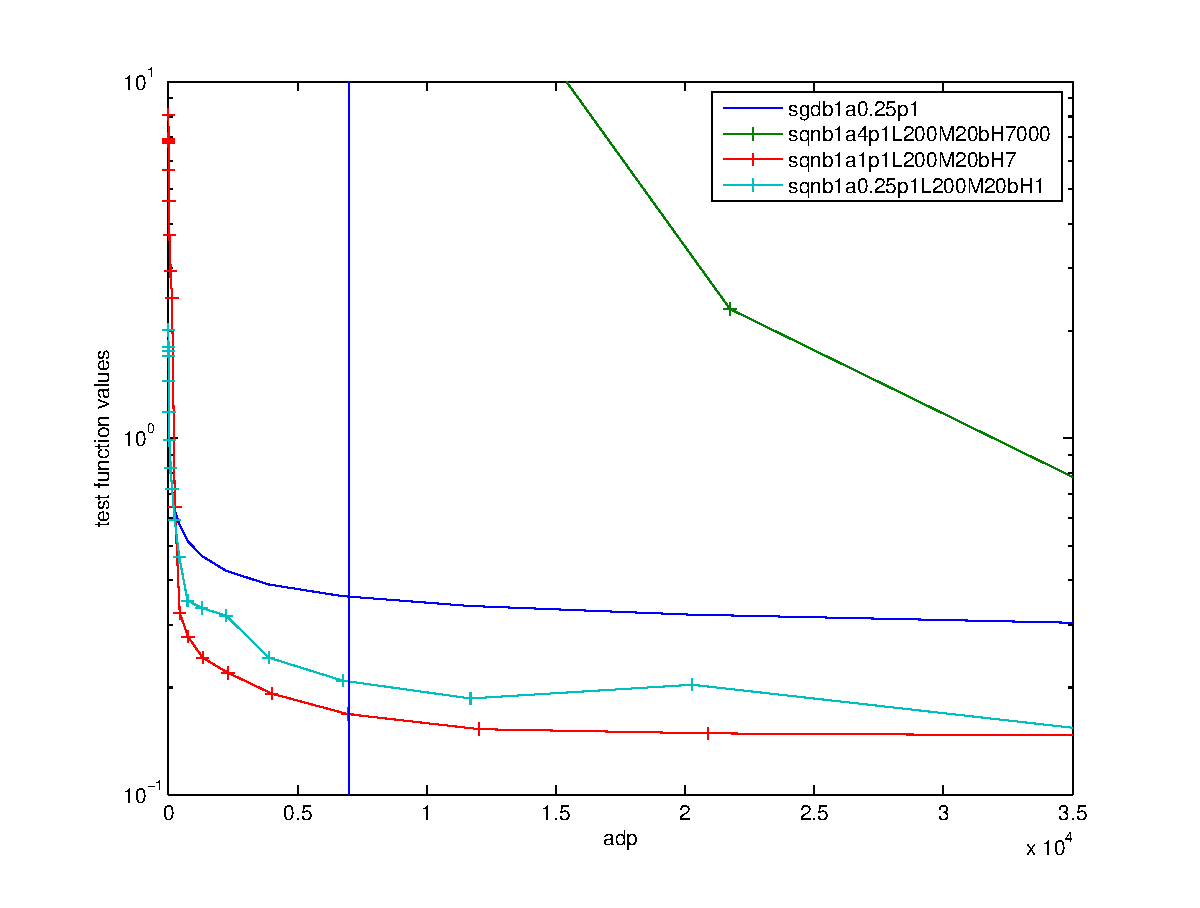
\includegraphics[scale=0.4]{figures/P02b.eps}
\end{frame}
\begin{frame}
	\frametitle{Performance - Speech}
	Compare sgd vs SQN by work
\end{frame}
\begin{frame}
	\frametitle{Performance - RCV1 - binary}
	Compare sgd vs SQN by work
\end{frame}
\begin{frame}
	\frametitle{Performance - RCV1 - tf-idf}
	Compare sgd vs SQN by work
\end{frame}
\begin{frame}
	\frametitle{Performance - RCV1 - tf-idf}
	Compare sgd vs SQN by work
\end{frame}

\begin{frame}
	\frametitle{Other Methods For Estimating Curvature}
	Discuss adagrad, gauss newton. What they do, how different, etc.
\end{frame}


\begin{frame}
	\frametitle{Nice, but what about other choices for matrix}
	Discuss adagrad, gauss newton. What they do, how different, etc.
\end{frame}

\begin{frame}
	\frametitle{AdaGrad}
	Full AdaGrad: at each iteration
	\begin{align*}
	 G_t &= G_{t-1}+ g_t  g_t^T\\
	 H_t &= \delta I + G_t^{1/2}\\
	 x_{t+1} &= x_{t} - \alpha_t H_t^{-1} g_t
	\end{align*}
	Update cost $>>O(n^2)$
	
	Diagonal AdaGrad:  at each iteration
	\begin{align*}
     s_{k,i} &=\sqrt{ ((k-1) s_{k-1,i})^2 +g_{k,i}^2 }, \quad i=1, \cdots, n \\
     H_k &=\delta I + diag(s_k) \\
	 x_{t+1} &= x_{t} - \alpha_t H_t^{-1} g_t
	\end{align*}
	Update cost $O(n)$
	
	For both implementations there is a parameter $\delta$ that might need tuning. Claim by authors that a tiny value works well. 
\end{frame}


\begin{frame}
	\frametitle{Natural Gradient}
	Full Memory: at each iteration
	\begin{align*}
	 H_{t} = \frac{t-1}{t}G_{t-1} + \frac{1}{t} g_{t-1} g_{t-1}^T \\
	 x_{t+1} &= x_{t} - \alpha_t H_t^{-1} g_t
	\end{align*}
	Update cost $O(n^2)$
	
	Limited Memory: at each iteration
	\begin{align*} 
	 H_{t} = \frac{t-1}{t}G_{t-1} + \frac{1}{t} g_{t-1} g_{t-1}^T\\
	 x_{t+1} &= x_{t} - \alpha_t H_t^{-1} g_t
	\end{align*}
	Update cost $O(n)$
\end{frame}

\begin{frame}
	\frametitle{Performance - Yoram }
	\includegraphics[scale=0.4]{figures/P01.eps}
	This is not encouraging, BUT, our algorithm is more general!
\end{frame}

\begin{frame}
	\frametitle{Why is $gg^T$ so good?}
	Say the optimization problem is actually
		\[
			\min_{\theta} \mathbb{E}_{(x,y)}[ f(\langle \theta, \Phi(x) \rangle,y)]
		\]
		The gradient is given by 
		\[
			 \mathbb{E}_{(x,y)}[  \Phi(x) \nabla f(\langle \theta, \Phi(x) \rangle,y)]
		\]
		The Hessian is
		\[
			 \mathbb{E}_{(x,y)}[  \Phi(x) \Phi(x)^T \nabla^2 f(\langle \theta, \Phi(x) \rangle,y)]
		\]
\end{frame}

\begin{frame}
	\frametitle{Why is $gg^T$ so good?}
	Say the optimization problem is actually
		\[
			\min_{\theta} \frac{1}{m} \sum_{i=1}^{m} f(\langle \theta, \Phi(x_i) \rangle,y_i)]
		\]
		The gradient is given by 
		\[
			  \frac{1}{m} \sum_{i=1}^{m} \Phi(x_i)  \nabla f(\langle \theta, \Phi(x_i) \rangle,y_i)] = \frac{1}{m} \sum_{i=1}^{m} g_i(\theta)  
		\]
		The Hessian is 
		\[
			  \frac{1}{m} \sum_{i=1}^{m} \Phi(x_i)  \Phi(x_i)^T  \nabla^2 f(\langle \theta, \Phi(x_i) \rangle,y_i)] =g_i(\theta)g_i^T(\theta)  
		\]
\end{frame}

\begin{frame}
	\frametitle{Not All Problems Have This Form!}
	   Multi-class logistic regression - the Speech problem.
\end{frame}

\begin{frame}
	\frametitle{Not All Problems Have This Form!}
	   A random quadratic
	   \[
	   		\min_{\theta}\mathbb{E}_{A,b}[\frac{1}{2}\theta^T A \theta - b^T \theta]
	   \]
	   \begin{itemize}
	   	\item Silly, because averaging samples $A_i$, $b_i$ $i \in {1,\ldots,m}$ can compute full batch gradients in same time as single example gradients
	   	\item Hessian is NOT a multiple of $g g^T$ 
	   \end{itemize}
\end{frame}


							 \begin{frame}
							 	\frametitle{a}
							 				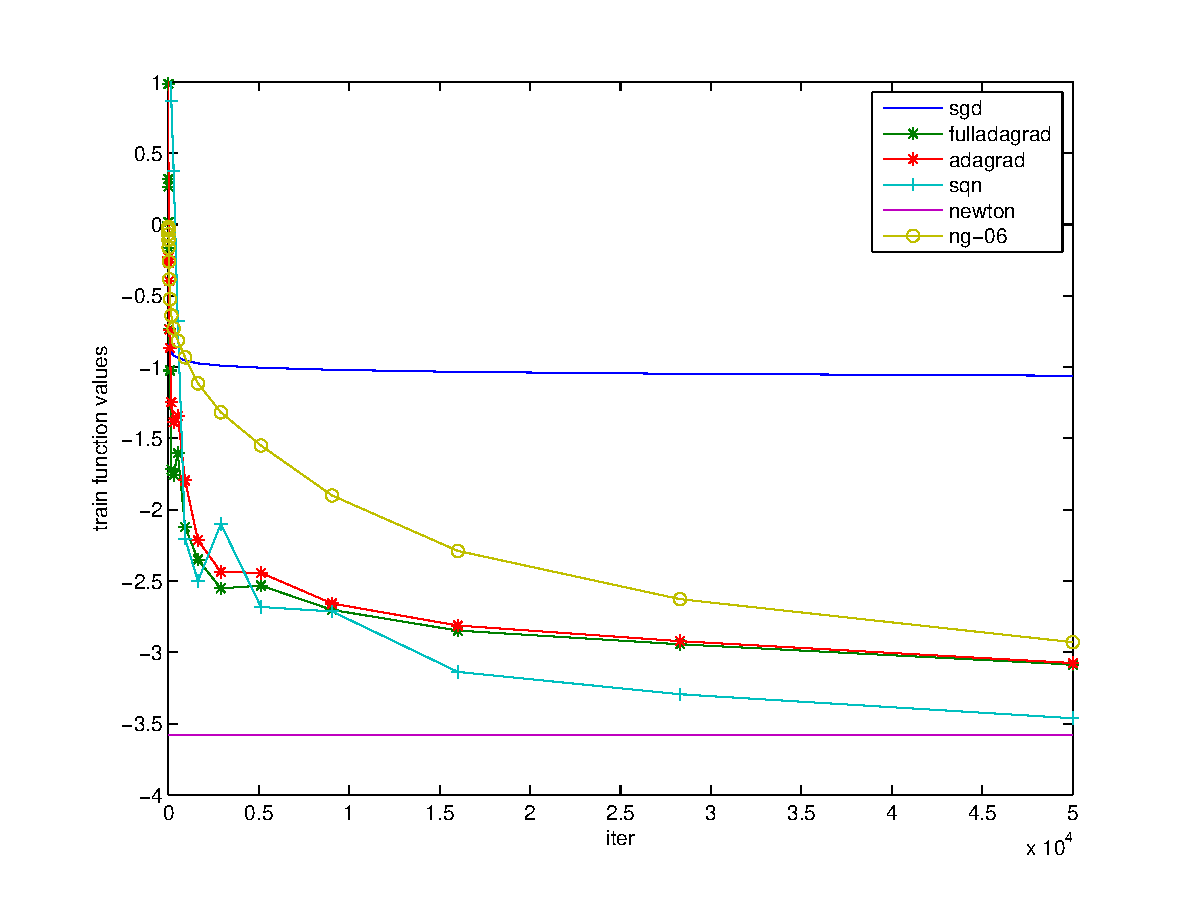
\includegraphics[scale=1]{figures/q.eps}
							 \end{frame} 
							 

\begin{frame}
	\frametitle{Performance - Others }
	Compare with diagonal adagrad and limited memory natural gradient
\end{frame}

\begin{frame}
	\frametitle{Conclusion}
	Other methods DO NOT outperform putting the true (computable) newton matrix. 
	
\end{frame}

\begin{frame}
	\frametitle{Where else can SQN be used? Beyond SGD}
	Averaged SGD, accelerated methods
\end{frame}

\begin{frame}
	\frametitle{Performance}
	Averaged SGD, accelerated methods
\end{frame}


\begin{frame}
	\frametitle{Costs}
	Compare with updating the gauss newton - say that we attempt to keep the costs linear in the dimension.
\end{frame}


\begin{frame}
	\frametitle{Costs - Cannot even work with full matrix $H^{-1}$}
	\[
	w_{t+1} \leftarrow w_{t} - \alpha_k H^{-1} g_t
	\]
	Approximations: diagonal, low rank, online L-BFGS
\end{frame}
 

	\begin{frame}
		\frametitle{Natural Gradient}
		\[
			G_{t+1} = \frac{t-1}{t}G_t + \frac{1}{t} g g^T
		\]
		Requires $O(n^2)$ computation 
	\end{frame}
	

	\begin{frame}
		\frametitle{Natural Gradient - Low memory verison}
		\[
			G_{t+1} = \frac{1}{K} \sum{i=t-K}^{t} g g^T 
		\]
	\end{frame}

	\begin{frame}
		\frametitle{Beyond SG}
		Averaged SGD - not clear if benefits from second order information\\
		"achieve the same rate of convergence as the optimal unimplementable algorithm" (Polyak, Juditsky 1992)
		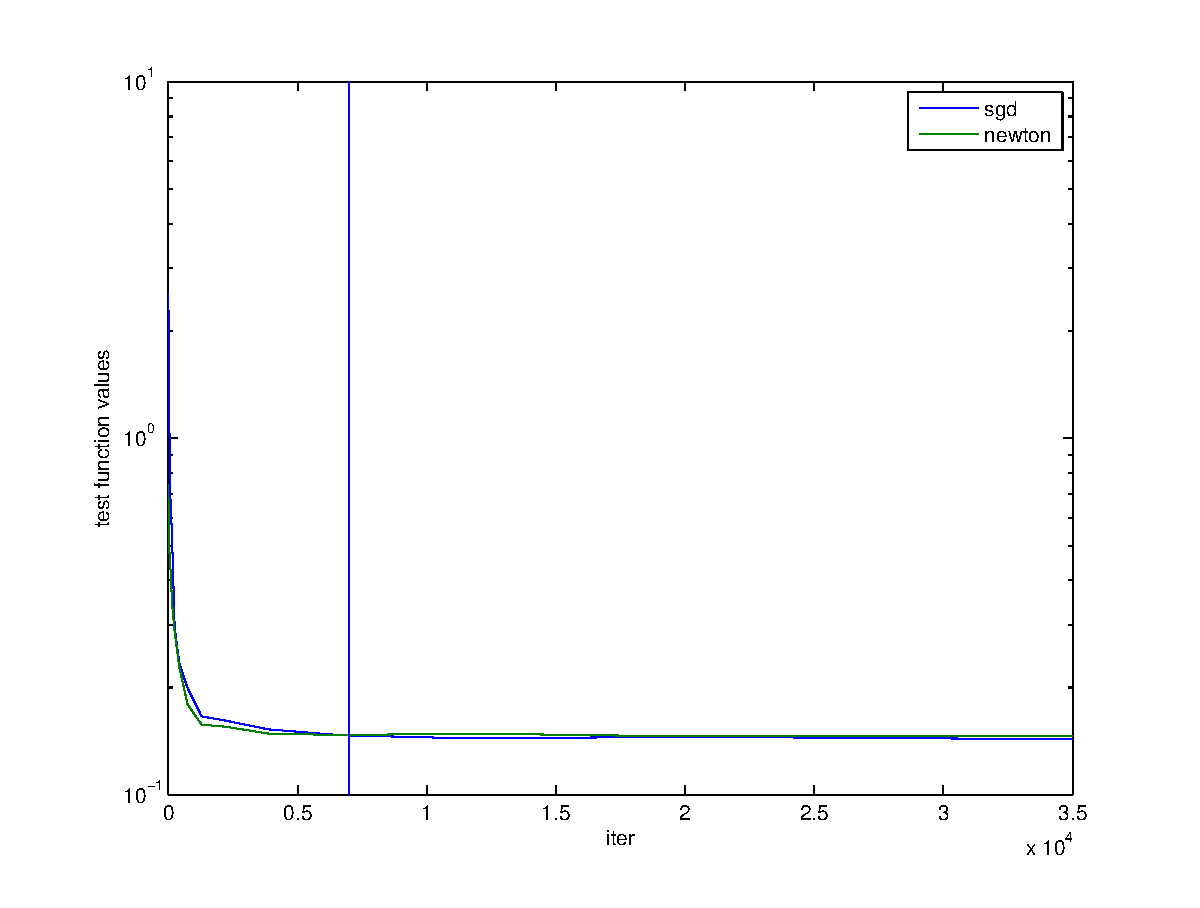
\includegraphics[scale=0.4]{figures/P03.eps}
	\end{frame}

	\begin{frame}
		\frametitle{Beyond SG}
		Dual Averaging - can also benefit from second order information. 
		Follow AdaGrad
	\end{frame}
	
	
	
	\begin{frame}

		\frametitle{Other directions}
		Say that for nonsmooth regularizers, such as $L1$ there is much potential, but too many good methods exist - if we focus on one we could get an algorithm. 

		Talk about L1 regularization, say that it would be nice to use SQN here. 
		Say first need to gain good understanding of methods for L1, describe deterministic methods, and where/which ones use second order information
		Speculate on how to adapt them to a stochastic setting
		\end{frame}
	
	
	\begin{frame}
		\frametitle{Problem - Quadratic $\ell_1$}
	\begin{equation*}
		\min_{x \in \mathbb{R}^n} \ F(x) = \frac{1}{2}x^T A x - b^T x +\tau \|x\|_1 ,
	\end{equation*}
		\end{frame}

	\begin{frame}
		\frametitle{Features of Proposed Method}
		\begin{itemize}
		\item Incorporates second-order information about the function $F$ through an inner conjugate gradient iteration \\
		\pause \item An active set method with a unique termination criteria for the subspace solve \\
		\begin{itemize}
		\item NOT an accuracy criteria. We do not have a pre-defined accuracy which, once reached, terminates the subspace solve.
		\item Automatically solve to high accuracy when a good subproblem is identified. 
		\end{itemize}
		\end{itemize}
	\end{frame}
	


	\begin{frame}
		\frametitle{"Inexact Second-order"}
		\begin{itemize}
			\item If it were an exact method, we would be solving the subproblems to optimality
			\begin{itemize}
				\item Either just reduce dimensionality, but still have a subproblem of the form $F$
				\item Or create a quadratic model and minimize until optimality, but this can be costly and unnecessary
			\end{itemize}
			\item Instead, 
		\end{itemize}
	\end{frame}
	\begin{frame}
		\frametitle{Active set for $F$}
		Active sets for constrained problems:
		\begin{itemize}
		\item Constraints which are active (satsfied with equality)
		\end{itemize}
		For an active set for an unconstrained nonsmooth function $F$ there is more than one choice
		\begin{itemize}
		\item Reformulate as a bound constrained QP, and use classical active set definition. This would force positive variables to stay nonegative, negative to stay nonpositive, and zero to stay zero. \\
		\item Another choice is less restrictive. Define an active set only by the zero variables: if it is zero, then it stays zero.
		\end{itemize}
	\end{frame}
	
	
	\begin{frame}
		\frametitle{Approximate Second Order Information}
		Using it exactly would mean computing $Ax=b$. 
		We don't fully compute such a Newton step. Instead use CG. 
		Our inexactness criteria is to terminate when leaving the subspace is beneficial, but more importantly if the function value is increasing. 
		\end{frame}
	
	
	\begin{frame}
		\frametitle{Known Methods That Use Second Order Information}
			First order methods
			Active Set Methods
			Interior point
			Scaled subgradient
		\end{frame}
	
	\begin{frame}
		\frametitle{Common inexactness criteria for }
			First order methods
			Active Set Methods
			Interior point
			Scaled subgradient
		\end{frame}
	

	\begin{frame}
		\frametitle{Problem - Quadratic $\ell_1$}
		This presentation will focus on a method for solving the following optimization problem:
		\begin{equation*}
			\min_{x \in \mathbb{R}^n} \ F(x) = \frac{1}{2}x^T A x - b^T x +\tau \|x\|_1 ,
		\end{equation*}
		where $A$ is a positive (semi)definite matrix, and $\tau$ is a regularization parameter.\\
		\pause This problem is of interest for sparse optimization, can be useful for machine learning, statistics, and other areas.
	\end{frame}


	\begin{frame}
	                                            \frametitle{Convergence: Linear Rate}
	\begin{theorem}
	\label{thm:qlinear} 
	Let $x^{k+1}$ be computed by either a proximal gradient step with $\frac{1}{16L} \leq \bar{\alpha} \leq \frac{1}{L}$, relaxation, or an accepted (not cut back) CG step. Then 
	\begin{equation*}
	F(x^{k+1}) - F^* \leq (1-\frac{\lambda}{16 L}) (F(x^k) - F^*).
	  \end{equation*}
	where $F^*$ is the optimal objective value. 
	\end{theorem}
	                                 \end{frame} 
        
	        \begin{frame}
	                                                    \frametitle{Convergence: Work Complexity}
	      Thus a work complexity result is possible as well. 
	    \begin{corollary}
	    The work complexity (number of matrix vector products) to reach $\epsilon$ accuracy in the objective value is 
	 \begin{equation*}
	  \frac{ 2 \log \{\frac{\epsilon}{(F(x^0) - F^*} \}}{\log\{ \sqrt{1-\frac{\lambda}{16 L}}\} }. 
	   \end{equation*}
	\end{corollary}
	                         \end{frame}
							 
							 
							 

							 \begin{frame}
							 	\frametitle{a}
							 				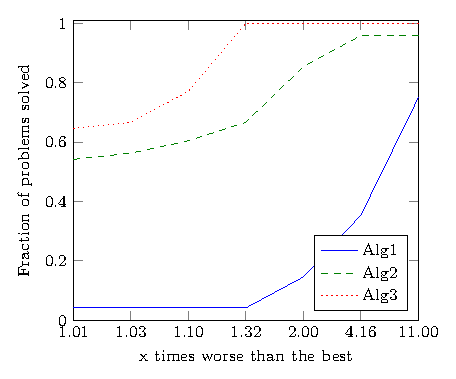
\includegraphics[scale=1]{figures/Fig1.eps}
							 \end{frame}
							 \begin{frame}
							 	\frametitle{a}
							 				\includegraphics[scale=1]{figures/Fig2a.eps}
							 \end{frame}
							 \begin{frame}
							 	\frametitle{a}
							 				\includegraphics[scale=1]{figures/Fig2b.eps}
							 \end{frame}
							 \begin{frame}
							 	\frametitle{a}
							 				\includegraphics[scale=1]{figures/Fig3a.eps}
							 \end{frame}
							 \begin{frame}
							 	\frametitle{a}
							 				\includegraphics[scale=1]{figures/Fig3b.eps}
							 \end{frame}
							 \begin{frame}
							 	\frametitle{a}
							 				\includegraphics[scale=1]{figures/Fig4a.eps}
							 \end{frame}
							 \begin{frame}
							 	\frametitle{a}
							 				\includegraphics[scale=1]{figures/Fig4b.eps}
							 \end{frame}
							 \begin{frame}
							 	\frametitle{a}
							 				\includegraphics[scale=1]{figures/Fig5a.eps}
							 \end{frame}
							 \begin{frame}
							 	\frametitle{a}
							 				\includegraphics[scale=1]{figures/Fig5b.eps}
							 \end{frame}
							 \begin{frame}
							 	\frametitle{a}
							 				\includegraphics[scale=1]{figures/Fig6a.eps}
							 \end{frame}
							 \begin{frame}
							 	\frametitle{a}
							 				\includegraphics[scale=1]{figures/Fig6b.eps}
							 \end{frame}
							 \begin{frame}
							 	\frametitle{a}
							 				\includegraphics[scale=1]{figures/Fig7a.eps}
							 \end{frame}
							 \begin{frame}
							 	\frametitle{a}
							 				\includegraphics[scale=1]{figures/Fig7b.eps}
							 \end{frame}
							 \begin{frame}
							 	\frametitle{a}
							 				\includegraphics[scale=1]{figures/Fig8a.eps}
							 \end{frame}
							 \begin{frame}
							 	\frametitle{a}
							 				\includegraphics[scale=1]{figures/Fig8b.eps}
							 \end{frame}
							 \begin{frame}
							 	\frametitle{a}
							 				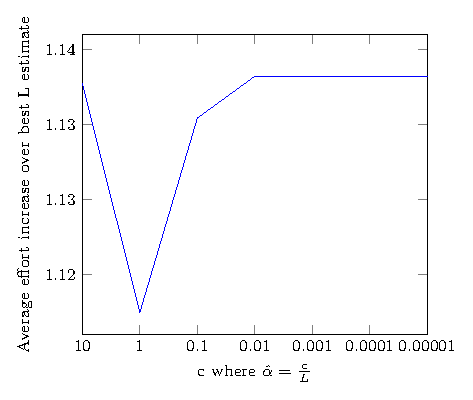
\includegraphics[scale=1]{figures/Fig9.eps}
							 \end{frame} 

							 \begin{frame}
							 	\frametitle{a}
							 				\includegraphics[scale=1]{figures/1.eps}
							 \end{frame} 
							 
							 
							 
							 
							 
							 
							 
							 
							 
							 
\end{document}